\documentclass{beamer}[10]

\usepackage{graphicx}
\usepackage{xcolor}
\usepackage{tabto}
%\usepackage{beamerthemesplit}
\usepackage{tikz}
\usepackage{cancel}
\usepackage{verbatim}
\usepackage{fancybox}
\usepackage{enumerate}
\usepackage{amsmath,amssymb,amsthm,textcomp,mathtools}
\usepackage[super]{nth}
\usepackage[amssymb]{SIunits}
\usepackage{booktabs}
\usepackage{cancel}
\usepackage{bm}
\usepackage[utf8]{inputenc}
\usepackage{tabularx}
\usepackage{ragged2e}
\newcolumntype{Y}{ >{\RaggedRight\arraybackslash}X}
\usetikzlibrary{arrows,shapes}
\newcommand\T{\rule{0pt}{2.6ex}}
\newcommand\B{\rule[-1.2ex]{0pt}{0pt}}
\definecolor{UUcrimson}{RGB}{204,0,0}
\mode<presentation>
{ \usetheme{default}
  \usecolortheme[named=UUcrimson]{structure}
  \useinnertheme{circles}
  \setbeamercovered{transparent}
  \setbeamertemplate{blocks}[rounded]
  \usefonttheme[onlymath]{serif}
  \setbeamertemplate{navigation symbols}{}
  \setbeamertemplate{footline}[page number]
  \setbeamertemplate{navigation symbols}{}
  \setbeamercolor{section in toc}{fg=black,bg=white}
  \setbeamercolor{alerted text}{fg=UUcrimson!80!gray}
  \setbeamercolor*{palette primary}{fg=white,bg=UUcrimson}
  \setbeamercolor*{palette secondary}{fg=UUcrimson!70!black,bg=gray!15!white}
  \setbeamercolor*{palette tertiary}{bg=UUcrimson!80!black,fg=gray!10!white}
  \setbeamercolor*{palette quaternary}{fg=UUcrimson,bg=gray!5!white}
  \setbeamercolor*{palette sidebar primary}{fg=UUcrimson!10!black}
  \setbeamercolor*{palette sidebar secondary}{fg=white}
  \setbeamercolor*{palette sidebar tertiary}{fg=UUcrimson!50!black}
  \setbeamercolor*{palette sidebar quaternary}{fg=gray!10!white}
  \setbeamercolor{titlelike}{parent=palette primary,fg=white}
  \setbeamercolor{frametitle}{bg=UUcrimson}
  \setbeamercolor{frametitle right}{bg=UUcrimson}
  \setbeamercolor*{separation line}{}
  \setbeamercolor*{fine separation line}{}
}

\usetikzlibrary{backgrounds}
\makeatletter
\tikzstyle{every picture}+=[remember picture]
\tikzset{%
  fancy quotes/.style={
    text width=\fq@width pt,
    align=justify,
    inner sep=1em,
    anchor=north west,
    minimum width=\linewidth,
    font=\itshape
  },
  fancy quotes width/.initial={.8\linewidth},
  fancy quotes marks/.style={
    scale=8,
    text=white,
    inner sep=0pt,
  },
  fancy quotes opening/.style={
    fancy quotes marks,
  },
  fancy quotes closing/.style={
    fancy quotes marks,
  },
  fancy quotes background/.style={
    show background rectangle,
    inner frame xsep=0pt,
    background rectangle/.style={
      fill=gray!25,
      rounded corners,
    },
  }
}
\newenvironment{fancyquotes}[1][]{%
\noindent
\tikzpicture[fancy quotes background]
\node[fancy quotes opening,anchor=north west] (fq@ul) at (0,0) {``};
\tikz@scan@one@point\pgfutil@firstofone(fq@ul.east)
\pgfmathsetmacro{\fq@width}{\linewidth - 2*\pgf@x}
\node[fancy quotes,#1] (fq@txt) at (fq@ul.north west) \bgroup}
{\egroup;
\node[overlay,fancy quotes closing,anchor=east] at (fq@txt.south east) {''};
\endtikzpicture}
\makeatother

\usepackage{scalerel}[2014/03/10]
\usepackage{stackengine}
\usepackage{empheq}
\newcommand*\widefbox[1]{\fbox{\hspace{0.5em}#1\hspace{0.5em}}}

\newcommand\reallywidetilde[1]{\ThisStyle{%
  \setbox0=\hbox{$\SavedStyle#1$}%
  \stackengine{-.1\LMpt}{$\SavedStyle#1$}{%
    \stretchto{\scaleto{\SavedStyle\mkern.2mu\sim}{.5467\wd0}}{.4\ht0}%
%    .2mu is the kern imbalance when clipping white space
%    .5467++++ is \ht/[kerned \wd] aspect ratio for \sim glyph
  }{O}{c}{F}{T}{S}%
}}
\usepackage{media9}

\logo{
\includegraphics[width=0.75cm]{logo.jpg}}
\author[Gibbs]{Dr. Jeremy A. Gibbs}
\institute{Department of Mechanical Engineering\\University of Utah}
\date{Fall 2016}
\title{LES of Turbulent Flows: Lecture 7}
\begin{document}

%----------------------------------------------------------------------------------------
%	TITLE & TOC SLIDES
%----------------------------------------------------------------------------------------

\begin{frame} 
  \titlepage
\end{frame}

%------------------------------------------------

\begin{frame}
\frametitle{Overview}
\tableofcontents
\end{frame}

%------------------------------------------------
\section{Recap of LES filtered equations for incompressible flows} %
%------------------------------------------------

\begin{frame}{LES filtered equations for incompressible flows}
Mass
\begin{itemize}
	\item $\frac{\partial \tilde u_i}{\partial x_i} = 0$
\end{itemize}

Momentum
\begin{itemize}
\item $\frac{\partial \tilde u_i}{\partial t} + \frac{\partial (\tilde u_i \tilde u_j)}{\partial x_j} = - \frac{\partial \tilde p}{\partial x_i} + \frac{1}{Re} \frac{\partial^2 \tilde u_i}{\partial x_j^{2}} -\frac{\partial \tau_{ij}}{\partial x_j}+ F_i$
\end{itemize}

Scalar
\begin{itemize}
	\item $\frac{\partial \tilde \theta}{\partial t} + \frac{\partial (\tilde u_i \tilde \theta)}{\partial x_j} = \frac{1}{Sc\ Re} \frac{\partial^2 \tilde \theta}{\partial x_j^{2}} -\frac{\partial q_i^r}{\partial x_j}+ Q$
\end{itemize}

SFS stress
\begin{itemize}
	\item $\tau_{ij}^r = \widetilde{u_i u_j} - \tilde u_i \tilde u_j$
\end{itemize}

SFS flux
\begin{itemize}
	\item $q_{i}^r = \widetilde{u_i \theta} - \tilde u_i \tilde \theta$
\end{itemize}
\end{frame}

%------------------------------------------------

\begin{frame}{Up next, turbulence kinetic energy}

\begin{itemize}
\item We've talked about variance (or energy) when discussing turbulence and filtering.
\item When we examined the application of the LES filter at scale $\Delta$ we saw the effect of the filter on the distribution of energy with scale.
\item A natural way to extend our examination of scale separation and energy is to look at the evolution of the filtered variance or turbulence kinetic energy.
\end{itemize}

\end{frame}

%------------------------------------------------
\section{The filtered kinetic energy equation for incompressible equations} %
%------------------------------------------------

\begin{frame}{The filtered kinetic energy equation}

\begin{itemize}
\item We can define the total filtered kinetic energy as
$$\tilde E = \frac{1}{2}\widetilde{u_i u_i}$$
\item Next we decompose this in the standard way as:
$$\tilde E = \underbrace{\tilde E_f}_{\substack{\text{Resolved}\\ \text{kinetic}\\\text{energy}}} + \underbrace{k_r}_{\substack{\text{SFS}\\\text{kinetic}\\\text{energy}}}$$
\item The SFS kinetic energy (residual kinetic energy) is defined as:
$$k_r = \frac{1}{2}\left(\widetilde{u_i u_i} - \tilde u_i \tilde u_i\right)$$
\end{itemize}

\end{frame}

%------------------------------------------------

\begin{frame}{The filtered kinetic energy equation}

\begin{itemize}
\item Putting them together yields:
$$\frac{1}{2}\widetilde{u_i u_j} = \tilde{E_f} + \frac{1}{2}\left(\widetilde{u_i u_i} - \tilde u_i \tilde u_i\right)$$
Thus the resolved (filtered) kinetic energy is then given by:
$$\tilde{E_f} = \frac{1}{2}\tilde u_i \tilde u_i$$
\end{itemize}

\end{frame}

%------------------------------------------------

\begin{frame}{The filtered kinetic energy equation}

\begin{itemize}
\item We can develop an equation for $\tilde E_f$ by multiplying the filtered LES momentum equation by $\tilde u_i$:
$$\underbrace{\tilde u_i\frac{\partial \tilde u_i}{\partial t}}_{\text{1}} + \underbrace{\tilde u_i\frac{\partial (\tilde u_i \tilde u_j)}{\partial x_j}}_{\text{2}} = \underbrace{- \tilde u_i\frac{\partial \tilde p}{\partial x_i}}_{\text{3}} + \underbrace{\frac{\tilde u_i}{Re} \frac{\partial^2 \tilde u_i}{\partial x_j^{2}}}_{\text{4}} \underbrace{-\tilde u_i\frac{\partial \tau_{ij}}{\partial x_j}}_{\text{5}}$$
\item The gist: we want to write the equation in terms of $\tilde E_f$. First we focus on terms (1)-(3) by applying the product rule, \textit{i.e.}
$$\frac{\partial (ab)}{\partial x} = a\frac{\partial b}{\partial x} + b\frac{\partial a}{\partial x}$$
\item Recall that the filtered rate of strain tensor is given by
$$\tilde S_{ij} = \frac{1}{2} \left(\frac{\partial \tilde u_i}{\partial x_j} + \frac{\partial \tilde u_j}{\partial x_i}\right)$$
\end{itemize}
\end{frame}

%------------------------------------------------

\begin{frame}{The filtered kinetic energy equation}

Term 1:
$$\frac{\partial (\tilde u_i \tilde u_i)}{\partial t} = \tilde u_i \frac{\partial \tilde u_i}{\partial t} + \tilde u_i \frac{\partial \tilde u_i}{\partial t} = 2\tilde u_i \frac{\partial \tilde u_i}{\partial t}$$
$$\Rightarrow \tilde u_i \frac{\partial \tilde u_i}{\partial t} = \frac{1}{2}\frac{\partial (\tilde u_i \tilde u_i)}{\partial t}$$
$$\boxed{\tilde u_i \frac{\partial \tilde u_i}{\partial t} = \frac{\partial \tilde E_f}{\partial t}}$$
\end{frame}

%------------------------------------------------

\begin{frame}{The filtered kinetic energy equation}
Term 2:
$$\text{first:}\qquad \tilde u_i\frac{\partial (\tilde u_i \tilde u_j)}{\partial x_j}=\tilde u_i \tilde u_i \cancelto{0 \text{ via continuity}}{\frac{\partial \tilde u_j}{\partial x_j}} + \tilde u_i \tilde u_j \frac{\partial \tilde u_i}{\partial x_j}$$
$$\text{next:}\qquad \tilde u_j\frac{\partial (\tilde u_i \tilde u_i)}{\partial x_j} = \tilde u_i \tilde u_j\frac{\partial \tilde u_i}{\partial x_j}+ \tilde u_i \tilde u_j\frac{\partial \tilde u_i}{\partial x_j} = 2\tilde u_i \tilde u_j\frac{\partial \tilde u_i}{\partial x_j}$$
$$\Rightarrow u_i \tilde u_j\frac{\partial \tilde u_i}{\partial x_j} = \frac{1}{2}\tilde u_j\frac{\partial (\tilde u_i \tilde u_i)}{\partial x_j}$$
$$\boxed{\tilde u_i\frac{\partial (\tilde u_i \tilde u_j)}{\partial x_j} = \tilde u_j\frac{\partial \tilde E_f}{\partial x_j}}$$
\end{frame}

%------------------------------------------------

\begin{frame}{The filtered kinetic energy equation}
Term 3:
$$\frac{\partial (\tilde u_i \tilde p)}{\partial x_i} = \tilde p \cancelto{0 \text{ via continuity}}{\frac{\tilde u_i}{\partial x_i}} + \tilde u_i\frac{\partial \tilde p}{\partial x_i}$$
$$\Rightarrow \boxed{\tilde u_i\frac{\partial \tilde p}{\partial x_j} = \frac{\partial (\tilde u_i \tilde p)}{\partial x_i}}$$
\end{frame}

%------------------------------------------------

\begin{frame}{The filtered kinetic energy equation}
Term 4:
$$\frac{\partial^2 (\tilde u_i \tilde u_i)}{\partial x_j^2} = \frac{\partial}{\partial x_j}\left[\frac{\partial (\tilde u_i \tilde u_i)}{\partial x_j}\right] =  \frac{\partial}{\partial x_j}\left[\tilde u_i\frac{\partial \tilde u_i}{\partial x_j} + u_i\frac{\partial \tilde u_i}{\partial x_j}\right]$$
$$\Rightarrow \frac{\partial}{\partial x_j}\left[2\tilde u_i\frac{\partial \tilde u_i}{\partial x_j}\right] = 2\frac{\partial \tilde u_i}{\partial x_j}\frac{\partial \tilde u_i}{\partial x_j} + 2 \tilde u_i \frac{\partial^2 \tilde u_i}{\partial x_j^2}$$
$$\frac{\tilde u_i}{\text{Re}} \frac{\partial^2 \tilde u_i}{\partial x_j^{2}} = \underbrace{\frac{1}{\text{Re}} \frac{\partial}{\partial x_j}\left[\tilde u_i\frac{\partial \tilde u_i}{\partial x_j}\right]}_{\text{4a}} - \underbrace{\frac{1}{\text{Re}}\frac{\partial \tilde u_i}{\partial x_j}\frac{\partial \tilde u_i}{\partial x_j}}_{\text{4b}}$$
\end{frame}

%------------------------------------------------

\begin{frame}{The filtered kinetic energy equation}

Term 4a:
$$\frac{1}{\text{Re}}\frac{\partial}{\partial x_j}\left[\tilde u_i\frac{\partial \tilde u_i}{\partial x_j}\right] = \frac{1}{\text{Re}}\frac{\partial}{\partial x_j}\left[\tilde u_i\frac{\partial \tilde u_i}{\partial x_j} + \tilde u_i\frac{\partial \tilde u_j}{\partial x_i} - \tilde u_i\frac{\partial \tilde u_j}{\partial x_i}\right]$$
$$= \frac{1}{\text{Re}}\frac{\partial (2\tilde u_i \tilde S_{ij})}{\partial x_j} - \frac{1}{\text{Re}}\frac{\partial}{\partial x_j} \left[\tilde u_i\frac{\partial \tilde u_j}{\partial x_i}\right]$$
$$=\frac{1}{\text{Re}}\frac{\partial (2\tilde u_i \tilde S_{ij})}{\partial x_j} - \frac{1}{\text{Re}}\frac{\partial \tilde u_i}{\partial x_j}\frac{\partial \tilde u_j}{\partial x_i} -  \frac{\tilde u_i}{\text{Re}}\cancelto{0 \text{ via continuity}}{\frac{\partial^2 \tilde u_j}{\partial x_j \partial x_i}}$$
$$= \frac{1}{\text{Re}}\frac{\partial (2\tilde u_i \tilde S_{ij})}{\partial x_j} - \frac{1}{\text{Re}}\frac{\partial \tilde u_i}{\partial x_j}\frac{\partial \tilde u_j}{\partial x_i}$$
\end{frame}

%------------------------------------------------

\begin{frame}{The filtered kinetic energy equation}

Combine terms 4a and 4b:
$$\frac{\tilde u_i}{\text{Re}} \frac{\partial^2 \tilde u_i}{\partial x_j^{2}} = \frac{1}{\text{Re}}\left[\frac{\partial (2\tilde u_i \tilde S_{ij})}{\partial x_j} - \frac{\partial \tilde u_i}{\partial x_j}\frac{\partial \tilde u_j}{\partial x_i} - \frac{\partial \tilde u_i}{\partial x_j}\frac{\partial \tilde u_i}{\partial x_j}\right]$$
This looks crazy. How do we reduce it further?
\end{frame}

%------------------------------------------------

\begin{frame}{The filtered kinetic energy equation}

Tensors:
\begin{itemize}
	\item Recall that any arbitrary \nth{2}-order tensor can be written as the sum of a symmetric and an antisymmetric tensor:
	$$\underbrace{B_{ij}}_{\text{arbitrary}} = \underbrace{S_{ij}}_{\text{symmetric}} + \underbrace{A_{ij}}_{\text{antisymmetric}}$$	
	\item Symmetric
	$$ S_{ij} = S_{ji}$$
	\item Antisymmetric
	$$ A_{ij} = -A_{ji}$$
\end{itemize}
\end{frame}

%------------------------------------------------

\begin{frame}{The filtered kinetic energy equation}

Tensors:
\begin{itemize}
	\item Proof:
	$$B_{ij} = \frac{1}{2}B_{ij} + \frac{1}{2}B_{ij} = \underbrace{\frac{1}{2}\left(B_{ij} + B_{ji}\right)}_{S_{ij}} + \underbrace{\frac{1}{2}\left(B_{ij} - B_{ji}\right)}_{A_{ij}} $$
	$$S_{ij} = \frac{1}{2}\left(B_{ij} + B_{ji}\right) = \frac{1}{2}\left(B_{ji} + B_{ij}\right) = S_{ji}$$
	$$A_{ij} = \frac{1}{2}\left(B_{ij} - B_{ji}\right) = -\frac{1}{2}\left(B_{ji} - B_{ij}\right) = -A_{ji}$$
\end{itemize}
\end{frame}

%------------------------------------------------

\begin{frame}{The filtered kinetic energy equation}

Tensors:
\begin{itemize}
	\item Let's apply this tensor idea
	$$\frac{\partial \tilde u_i}{\partial x_j} = \tilde S_{ij} + \tilde A_{ij} \qquad \text{and} \qquad \frac{\partial \tilde u_j}{\partial x_i} = \tilde S_{ji} + \tilde A_{ji}$$
	\item Using this
	$$\frac{\partial \tilde u_i}{\partial x_j}\frac{\partial \tilde u_i}{\partial x_j} =  \tilde S_{ij}\tilde S_{ij} + 2\tilde S_{ij}\tilde A_{ij} + \tilde A_{ij}\tilde A_{ij}$$
	$$\frac{\partial \tilde u_i}{\partial x_j}\frac{\partial \tilde u_j}{\partial x_i} = \tilde S_{ij}\tilde S_{ji} + \tilde S_{ij} \tilde A_{ji} + \tilde S_{ji} \tilde A_{ij} + \tilde A_{ij}\tilde A_{ji}$$
	\item Whoa, this is getting out of hand. Can we reduce these expressions?
\end{itemize}
\end{frame}

%------------------------------------------------

\begin{frame}{The filtered kinetic energy equation}

Tensors:
\begin{itemize}
	\item Let's look at a general property of symmetric/antisymmetric tensors:
	$$S_{ij}A_{ij} = -S_{ij}A{ji}$$
	Rename dummy variables and use symmetry
	$$-S_{ij}A{ji} = -S_{ji}A{ij} = -S_{ij}A{ij}$$
	Thus
	$$S_{ij}A_{ij} = -S_{ij}A{ij} \Rightarrow 2S_{ij}A_{ij}=0\Rightarrow S_{ij}A_{ij} = 0$$
	The product of a symmetric and antisymmetric tensor is 0.
\end{itemize}
\end{frame}

%------------------------------------------------

\begin{frame}{The filtered kinetic energy equation}

Tensors:
\begin{itemize}
	\item Back to our definitions
	$$\frac{\partial \tilde u_i}{\partial x_j}\frac{\partial \tilde u_i}{\partial x_j} =  \tilde S_{ij}\tilde S_{ij} + 2\cancelto{0}{\tilde S_{ij}\tilde A_{ij}} + \tilde A_{ij}\tilde A_{ij} = \tilde S_{ij}\tilde S_{ij} + \tilde A_{ij}\tilde A_{ij}$$
	$$\frac{\partial \tilde u_i}{\partial x_j}\frac{\partial \tilde u_j}{\partial x_i} = \tilde S_{ij}\tilde S_{ji} + \cancelto{0}{\tilde S_{ij} \tilde A_{ji}} + \cancelto{0}{\tilde S_{ji} \tilde A_{ij}} + \tilde A_{ij}\tilde A_{ji} = \tilde S_{ij}\tilde S_{ji} + \tilde A_{ij}\tilde A_{ji}$$
	Let's plug these expressions back into Term 4.
\end{itemize}
\end{frame}

%------------------------------------------------

\begin{frame}{The filtered kinetic energy equation}

Term 4:
\begin{align*}
\frac{\tilde u_i}{\text{Re}} \frac{\partial^2 \tilde u_i}{\partial x_j^{2}} &= \frac{1}{\text{Re}}\left[\frac{\partial (2\tilde u_i \tilde S_{ij})}{\partial x_j} - \frac{\partial \tilde u_i}{\partial x_j}\frac{\partial \tilde u_j}{\partial x_i} - \frac{\partial \tilde u_i}{\partial x_j}\frac{\partial \tilde u_i}{\partial x_j}\right]\\
&= \frac{1}{\text{Re}}\left[\frac{\partial (2\tilde u_i \tilde S_{ij})}{\partial x_j} - S_{ij}\tilde S_{ij} - \tilde A_{ij}\tilde A_{ij} - \tilde S_{ij}\tilde S_{ji} - \tilde A_{ij}\tilde A_{ji}\right]
\end{align*}
Note $S_{ji} = S_{ij}$ and $\tilde A_{ij}\tilde A_{ji} = -\tilde A_{ij}\tilde A_{ij}$
\begin{align*}
\hphantom{\frac{\tilde u_i}{\text{Re}} \frac{\partial^2 \tilde u_i}{\partial x_j^{2}}}	&= \frac{1}{\text{Re}}\left[\frac{\partial (2\tilde u_i \tilde S_{ij})}{\partial x_j} - S_{ij}\tilde S_{ij} - \cancelto{}{\tilde A_{ij}\tilde A_{ij}} - \tilde S_{ij}\tilde S_{ij} + \cancelto{}{\tilde A_{ij}\tilde A_{ij}}\right]\\
\Aboxed{&= \frac{2}{\text{Re}}\frac{\partial (\tilde u_i \tilde S_{ij})}{\partial x_j} - \underbrace{\frac{2}{\text{Re}}\tilde S_{ij}\tilde S_{ij}}_{\epsilon_f}}
\end{align*}

\end{frame}

%------------------------------------------------

\begin{frame}{The filtered kinetic energy equation}

\begin{itemize}
\item Term 5:
$$\frac{\partial (\tilde u_i \tau_{ij})}{\partial x_j}  = \tilde u_i \frac{\partial \tau_{ij}}{\partial x_j} + \tau_{ij} \frac{\partial \tilde u_i}{\partial x_j}$$
$$\boxed{\Rightarrow \tilde u_i\frac{\partial \tau_{ij}}{\partial x_j} = \frac{\partial (\tilde u_i \tau_{ij})}{\partial x_j} \underbrace{-\tau_{ij} \frac{\partial \tilde u_i}{\partial x_j}}_{\Pi=\tau_{ij}\tilde S_{ij}}}$$
Note: 
\begin{align*}
\tau_{ij} \frac{\partial \tilde u_i}{\partial x_j} &= \tau_{ij}(\tilde S_{ij} + \tilde A_{ij})= \tau_{ij} \tilde S_{ij} + \tau_{ij} \tilde A_{ij}\\
&= \tau_{ij} \tilde S_{ij} + \cancelto{\tau_{ij} = \widetilde{u_iu_j} - \tilde u_i \tilde u_j \text{ is symmetric}}{\tau_{ij} \tilde A_{ij}}\\
&= \tau_{ij} \tilde S_{ij}
\end{align*}
Now, let's put terms (1)-(5) back together.
\end{itemize}
\end{frame}

%------------------------------------------------

\begin{frame}{The filtered kinetic energy equation}
The dimensionless filtered TKE equation
$$\underbrace{\vphantom{ \tilde u_j\frac{\partial \tilde E_f}{\partial x_j}}  \frac{\partial \tilde E_f}{\partial t}}_{\text{I}} + \underbrace{\tilde u_j\frac{\partial \tilde E_f}{\partial x_j}}_{\text{II}} = -\underbrace{\vphantom{ \tilde u_j\frac{\partial \tilde E_f}{\partial x_j}}\frac{\partial (\tilde u_i \tilde p)}{\partial x_i}}_{\text{III}} - \underbrace{\vphantom{ \tilde u_j\frac{\partial \tilde E_f}{\partial x_j}}\frac{\partial (\tilde u_i \tau_{ij})}{\partial x_j}}_{\text{IV}} - \underbrace{\vphantom{ \tilde u_j\frac{\partial \tilde E_f}{\partial x_j}}\frac{2}{\text{Re}}\frac{\partial (\tilde u_i \tilde S_{ij})}{\partial x_j}}_{\text{V}} - \underbrace{\vphantom{ \tilde u_j\frac{\partial \tilde E_f}{\partial x_j}}\epsilon_f}_{\text{VI}} -\underbrace{\vphantom{ \tilde u_j\frac{\partial \tilde E_f}{\partial x_j}}\Pi}_{\text{VII}}$$

\begin{enumerate}[I]
\item ``storage'' of $\tilde E_f$
\item advection of $\tilde E_f$
\item pressure transport
\item transport of SFS stress $\tau_{ij}$
\item transport of viscous stress
\item dissipation by viscous stress
\item SFS dissipation
\end{enumerate}
\end{frame}

%------------------------------------------------

\begin{frame}{The filtered kinetic energy equation}
The dimensional filtered TKE equation
$$\underbrace{\vphantom{ \tilde u_j\frac{\partial \tilde E_f}{\partial x_j}}  \frac{\partial \tilde E_f}{\partial t}}_{\text{I}} + \underbrace{\tilde u_j\frac{\partial \tilde E_f}{\partial x_j}}_{\text{II}} = -\underbrace{\vphantom{ \tilde u_j\frac{\partial \tilde E_f}{\partial x_j}}\frac{1}{\rho} \frac{\partial (\tilde u_i \tilde p)}{\partial x_i}}_{\text{III}} - \underbrace{\vphantom{ \tilde  u_j\frac{\partial \tilde E_f}{\partial x_j}}\frac{\partial (\tilde u_i \tau_{ij})}{\partial x_j}}_{\text{IV}} - \underbrace{\vphantom{ \tilde u_j\frac{\partial \tilde E_f}{\partial x_j}}2\nu\frac{\partial (\tilde u_i \tilde S_{ij})}{\partial x_j}}_{\text{V}} - \underbrace{\vphantom{ \tilde u_j\frac{\partial \tilde E_f}{\partial x_j}}\epsilon_f}_{\text{VI}} -\underbrace{\vphantom{ \tilde u_j\frac{\partial \tilde E_f}{\partial x_j}}\Pi}_{\text{VII}}$$

where $\epsilon_f = 2\nu\tilde S_{ij} \tilde S_{ij}$.

\begin{enumerate}[I]
\item ``storage'' of $\tilde E_f$
\item advection of $\tilde E_f$
\item pressure transport
\item transport of SFS stress $\tau_{ij}$
\item transport of viscous stress
\item dissipation by viscous stress
\item SFS dissipation
\end{enumerate}

\end{frame}

%------------------------------------------------

\begin{frame}{Transfer of energy between resolved and SFSs}
\begin{itemize}
	\item The SFS dissipation $\Pi$ in the resolved kinetic energy equation is a sink of resolved kinetic energy (it is a source in the $k_r$ equation) and represents the transfer of energy from resolved SFSs. It is equal to:
	$$\Pi = -\tau_{ij} \tilde S_{ij}$$
	\item It is referred to as the SFS dissipation as an analogy to viscous dissipation (and in the inertial subrange $\Pi$ = viscous dissipation).
\end{itemize}
\end{frame}

%------------------------------------------------

\begin{frame}{Transfer of energy between resolved and SFSs}

\begin{figure}
	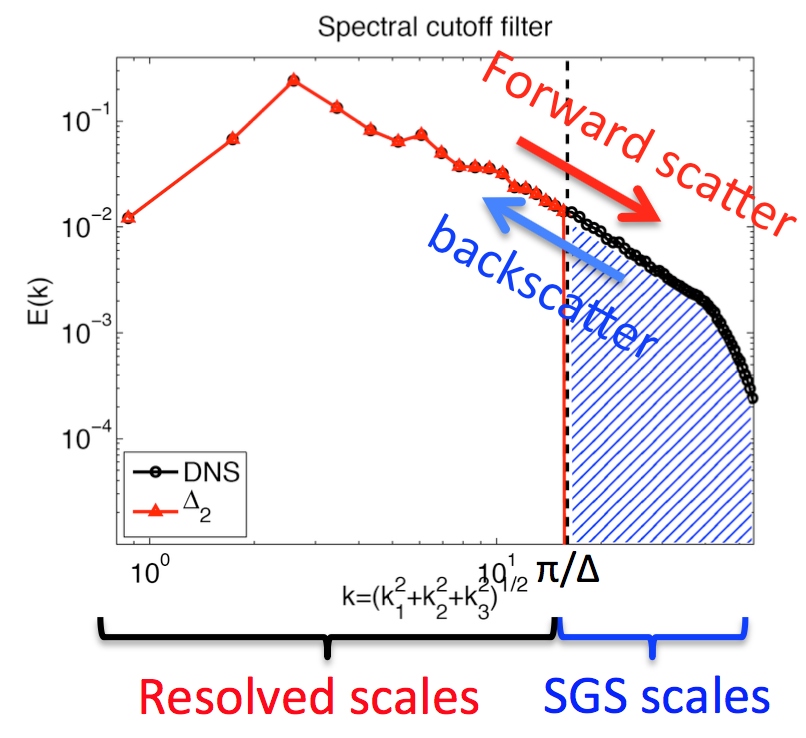
\includegraphics[width=0.55\textwidth]{scales.png}
\end{figure}
 \begin{itemize}
	\item \textit{On average}, $\Pi$ drains energy (transfers energy down to smaller scales) from the resolved scales.
	\item Instantaneously (locally) $\Pi$ can be positive or negative.
\end{itemize}
\end{frame}

%------------------------------------------------

\begin{frame}{Transfer of energy between resolved and SFSs}

\begin{figure}
	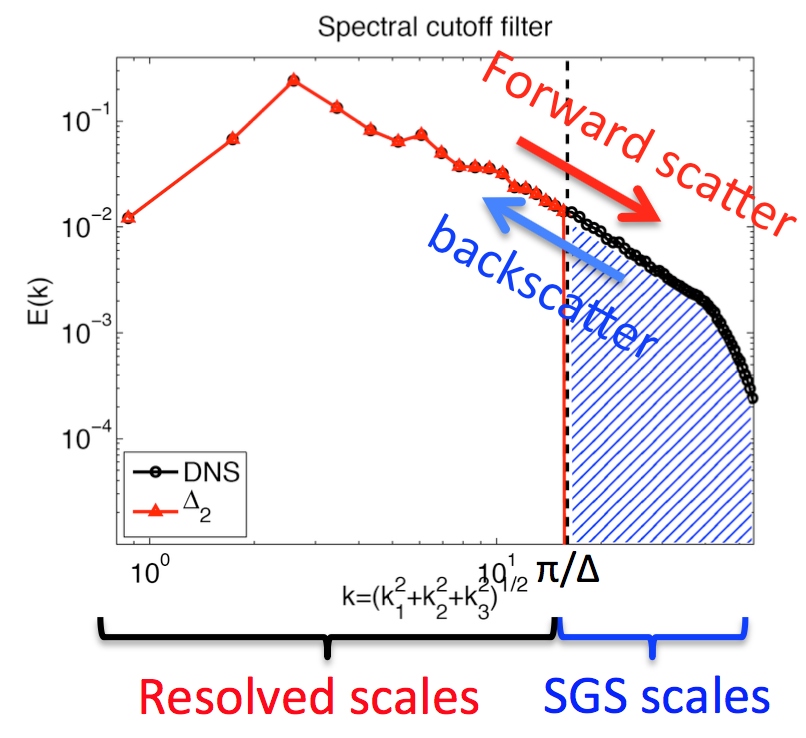
\includegraphics[width=0.55\textwidth]{scales.png}
\end{figure}
\begin{itemize}
	\item When $\Pi$ is negative (transfer from SFS $\Rightarrow$ resolved scales) it is typically termed backscatter
	\item When $\Pi$ is positive (transfer from resolved scales $\Rightarrow$ SFS) it is sometimes referred to as forward scatter.
\end{itemize}
\end{frame}

%------------------------------------------------

\begin{frame}{Transfer of energy between resolved and SFSs}

\begin{itemize}
	\item It is informative to compare our resolved kinetic energy equation to the mean kinetic energy equation (derived in a similar manner, see Pope pg. 124; Stull 1988 ch. 5)
	$$\frac{\partial \langle E\rangle}{\partial t} + \langle u_i\rangle \frac{\partial \langle E \rangle}{\partial x_j} = -\frac{1}{\rho} \frac{\partial \langle u_i\rangle \langle p \rangle}{\partial x_j} - \frac{\partial}{\partial x_j} 2\nu\langle u_i\rangle \langle S_{ij}\rangle -P - \langle \epsilon \rangle$$
	where $P$ is shear production and $\langle \epsilon \rangle$ is mean dissipation.
	$$P = \langle u_i^\prime u_j^\prime \rangle \frac{\partial \langle u_i\rangle}{\partial x_j}$$
	$$\langle \epsilon \rangle = 2\nu\langle S_{ij}\rangle \langle S_{ij}\rangle$$
\end{itemize}
\end{frame}

%------------------------------------------------

\begin{frame}{Transfer of energy between resolved and SFSs}
	$$\frac{\partial \tilde E_f}{\partial t} + \tilde u_j\frac{\partial \tilde E_f}{\partial x_j} = -\frac{1}{\rho} \frac{\partial (\tilde u_i \tilde p)}{\partial x_i} - \frac{\partial (\tilde u_i \tau_{ij})}{\partial x_j} - 2\nu\frac{\partial (\tilde u_i \tilde S_{ij})}{\partial x_j}- \epsilon_f -\Pi$$
	$$\frac{\partial \langle E\rangle}{\partial t} + \langle u_i\rangle \frac{\partial \langle E \rangle}{\partial x_j} = -\frac{1}{\rho} \frac{\partial \langle u_i\rangle \langle p \rangle}{\partial x_j} -P - 2\nu\frac{\partial}{\partial x_j} \langle u_i\rangle \langle S_{ij}\rangle - \langle \epsilon \rangle$$
\begin{itemize}
	\item For high-Re flow, with our filter in the inertial subrange: $\langle \tilde E_f \rangle = \langle E \rangle$
	\item The dominant sink for $\langle \tilde E_f \rangle$ is $\langle \Pi \rangle$ while for $\langle E \rangle$ it is $\langle \epsilon \rangle$ (rate of dissipation of energy). For high-Re flow we therefore have:
	$$\langle \Pi \rangle \approx \langle \epsilon \rangle$$
\end{itemize}
\end{frame}

%------------------------------------------------

\begin{frame}{Transfer of energy between resolved and SFSs}
	$$\frac{\partial \tilde E_f}{\partial t} + \tilde u_j\frac{\partial \tilde E_f}{\partial x_j} = -\frac{1}{\rho} \frac{\partial (\tilde u_i \tilde p)}{\partial x_i} - \frac{\partial (\tilde u_i \tau_{ij})}{\partial x_j} - 2\nu\frac{\partial (\tilde u_i \tilde S_{ij})}{\partial x_j}- \epsilon_f -\Pi$$
	$$\frac{\partial \langle E\rangle}{\partial t} + \langle u_i\rangle \frac{\partial \langle E \rangle}{\partial x_j} = -\frac{1}{\rho} \frac{\partial \langle u_i\rangle \langle p \rangle}{\partial x_j} -P - 2\nu\frac{\partial}{\partial x_j} \langle u_i\rangle \langle S_{ij}\rangle - \langle \epsilon \rangle$$
\begin{itemize}
	\item Recall from K41 that $\langle \epsilon \rangle$ is proportional to the transfer of energy in the inertial subrange. Thus, $\Pi$ will have a strong impact on energy transfer and the shape of the energy spectrum in LES.
	\item Calculating the correct average $\Pi$ is another necessary (but not sufficient) condition for an LES SFS model (to go with our N-S invariance properties).
\end{itemize}
\end{frame}


%------------------------------------------------

\end{document}

